\section{CNN Nhỏ gọn cho Edge AI: Hiệu quả trong Thế giới Thực}
\label{sec:compact_cnns_for_edge_ai}

Sự thành công của các kiến trúc CNN sâu như ResNet và EfficientNet trên các bộ dữ liệu quy mô lớn đã chứng minh sức mạnh của học sâu. Tuy nhiên, những mô hình này thường là những "gã khổng lồ" về mặt tính toán, với hàng chục, thậm chí hàng trăm triệu tham số, đòi hỏi các cụm GPU mạnh mẽ để huấn luyện và suy luận. Trong khi đó, cuộc cách mạng AI thực sự không chỉ diễn ra trên các đám mây (cloud), mà còn đang lan tỏa mạnh mẽ ra "vùng biên" (the edge).

\subsection{Bối cảnh và Nhu cầu của Trí tuệ Nhân tạo tại Biên (Edge AI)}
\label{subsec:edge_ai_context}
\textbf{Edge AI} là một mô thức trong đó các tác vụ AI được thực thi trực tiếp trên thiết bị cục bộ, thay vì gửi dữ liệu lên một máy chủ từ xa để xử lý. Các thiết bị này bao gồm tất cả mọi thứ xung quanh chúng ta: điện thoại thông minh, camera an ninh, drone, thiết bị đeo, loa thông minh, và thậm chí cả các cảm biến trong xe tự hành.

Việc thực thi AI tại biên mang lại những lợi ích to lớn:
\begin{itemize}
	\item \textbf{Độ trễ thấp (Low Latency):} Xử lý tại chỗ loại bỏ độ trễ của việc truyền dữ liệu qua mạng, điều tối quan trọng cho các ứng dụng thời gian thực như xe tự hành hay robot.
	\item \textbf{Bảo mật và Quyền riêng tư (Security \& Privacy):} Dữ liệu nhạy cảm (ví dụ: hình ảnh khuôn mặt) không cần phải rời khỏi thiết bị, giảm thiểu rủi ro về quyền riêng tư.
	\item \textbf{Hoạt động ngoại tuyến (Offline Operation):} Các thiết bị có thể tiếp tục hoạt động thông minh ngay cả khi không có kết nối Internet.
	\item \textbf{Tiết kiệm băng thông:} Giảm chi phí và gánh nặng cho cơ sở hạ tầng mạng.
\end{itemize}

Tuy nhiên, các thiết bị biên đi kèm với những ràng buộc phần cứng khắc nghiệt, hoàn toàn trái ngược với môi trường máy chủ lý tưởng:
\begin{itemize}
	\item \textbf{Công suất tiêu thụ thấp:} Thường hoạt động bằng pin, yêu cầu mức tiêu thụ năng lượng cực thấp (ví dụ: $\le 1$ Watt).
	\item \textbf{Bộ nhớ hạn chế:} RAM và bộ nhớ lưu trữ thường chỉ có vài trăm megabyte.
	\item \textbf{Năng lực tính toán giới hạn:} Các CPU/DSP/NPU di động có số lượng phép tính mỗi giây (FLOPS) thấp hơn nhiều so với GPU máy chủ.
\end{itemize}
Từ đó, một nhánh nghiên cứu quan trọng đã ra đời: thiết kế các kiến trúc CNN \textbf{nhỏ gọn và hiệu quả}, tối ưu hóa sự cân bằng tinh tế giữa độ chính xác, tốc độ suy luận, và chi phí tài nguyên.

\subsection{Các Nguyên lý Thiết kế Nền tảng cho CNN Nhẹ}
\label{subsec:lightweight_cnn_principles}
Để thu nhỏ một mạng CNN mà không làm suy giảm quá nhiều độ chính xác, các nhà nghiên cứu đã phát minh ra một loạt các khối xây dựng và nguyên lý thiết kế thông minh.

\subsubsection{Depthwise Separable Convolution}
\label{subsubsec:depthwise_separable_conv}
Đây là ý tưởng đột phá nhất, được giới thiệu trong Xception và phổ biến hóa bởi dòng họ MobileNet \cite{Howard2017}. Nó chia một phép tích chập 2D tiêu chuẩn thành hai bước riêng biệt:
\begin{enumerate}
	\item \textbf{Depthwise Convolution:} Áp dụng một bộ lọc 2D duy nhất cho mỗi kênh đầu vào một cách độc lập. Nếu input có $C_{in}$ kênh, bước này sẽ sử dụng $C_{in}$ bộ lọc 2D để tạo ra một output cũng có $C_{in}$ kênh. Nó chỉ thực hiện việc lọc không gian.
	\item \textbf{Pointwise Convolution:} Áp dụng một phép tích chập $1 \times 1$ thông thường để kết hợp thông tin từ các kênh được tạo ra ở bước depthwise. Bước này thực hiện việc kết hợp thông tin giữa các kênh.
\end{enumerate}

\begin{mdframed}[style=infobox]
	\textbf{Phân tích Hiệu quả Tính toán}
	
	Hãy so sánh chi phí tính toán (số phép nhân-cộng, MACs) giữa một phép tích chập tiêu chuẩn và một phép tích chập có thể tách rời. Giả sử input có kích thước $H \times W \times C_{in}$, output có kích thước $H \times W \times C_{out}$, và kernel có kích thước $F \times F$.
	\begin{itemize}
		\item \textbf{Standard Convolution:} $H \cdot W \cdot F \cdot F \cdot C_{in} \cdot C_{out}$
		\item \textbf{Depthwise Separable Conv:} $(H \cdot W \cdot F \cdot F \cdot C_{in}) + (H \cdot W \cdot 1 \cdot 1 \cdot C_{in} \cdot C_{out})$
	\end{itemize}
	Tỷ lệ giảm chi phí là:
	\begin{equation}
		\frac{\text{Cost}_{\text{separable}}}{\text{Cost}_{\text{standard}}} = \frac{H W F^2 C_{in} + H W C_{in} C_{out}}{H W F^2 C_{in} C_{out}} = \frac{1}{C_{out}} + \frac{1}{F^2}
	\end{equation}
	Với kernel $3 \times 3$ ($F=3$) và số kênh đầu ra lớn, tỷ lệ này xấp xỉ $1/F^2 = 1/9$. Tức là, Depthwise Separable Convolution có thể giảm chi phí tính toán xuống gần \textbf{8-9 lần} so với tích chập tiêu chuẩn với sự suy giảm độ chính xác không đáng kể.
\end{mdframed}

\begin{center}
	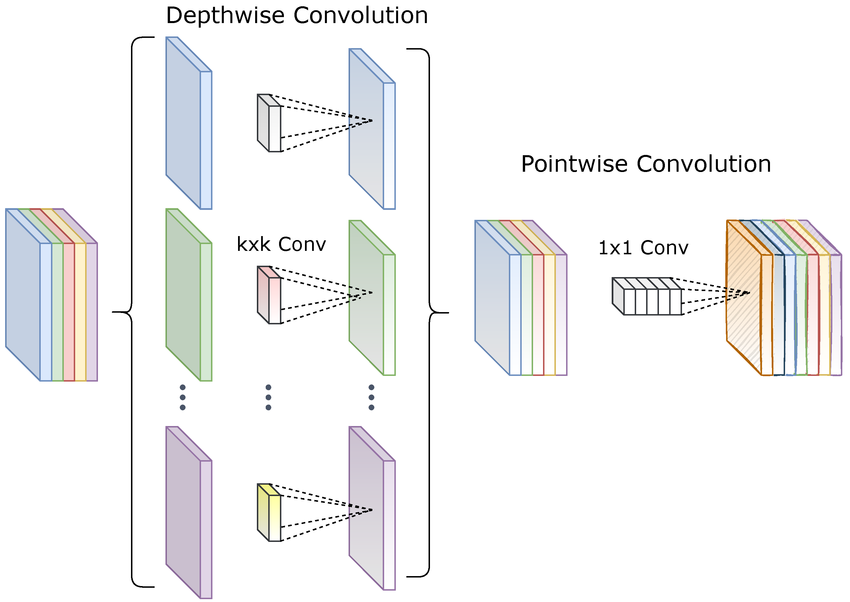
\includegraphics[width=1.0\textwidth]{images/depthwise_separable_convolution.png}
	\captionof{figure}{So sánh giữa Tích chập Tiêu chuẩn (phải) và Tích chập Tách rời theo Chiều sâu (trái). Phép toán được chia thành hai bước: Depthwise (lọc trên từng kênh) và Pointwise (kết hợp các kênh).}
	\label{fig:depthwise_separable_conv}
\end{center}
% Keyword gợi ý: depthwise separable convolution, standard vs depthwise convolution

\subsubsection{Inverted Residuals và Linear Bottleneck}
\label{subsubsec:inverted_residuals}
Được giới thiệu trong MobileNetV2 \cite{Sandler2018}, khối xây dựng này là một sự cải tiến quan trọng so với khối residual của ResNet.
\begin{itemize}
	\item \textbf{Inverted Residual:} Ngược lại với khối "bottleneck" của ResNet (nén-xử lý-mở rộng), khối này hoạt động theo chu trình \textbf{mở rộng-xử lý-nén}. Nó sử dụng một lớp $1 \times 1$ để mở rộng số kênh, sau đó áp dụng lớp Depthwise Conv $3 \times 3$ hiệu quả trên không gian đặc trưng nhiều chiều này, và cuối cùng dùng một lớp $1 \times 1$ khác để nén số kênh trở lại.
	\item \textbf{Linear Bottleneck:} Các tác giả phát hiện ra rằng việc sử dụng hàm kích hoạt phi tuyến (như ReLU) sau lớp nén cuối cùng sẽ làm mất mát thông tin quan trọng ở các không gian đặc trưng ít chiều. Do đó, lớp chiếu (projection) $1 \times 1$ cuối cùng này được giữ ở dạng tuyến tính (không có hàm kích hoạt).
\end{itemize}
Sự kết hợp này, cùng với các kết nối tắt (skip connections) tương tự ResNet, tạo ra một khối xây dựng vừa mạnh mẽ vừa hiệu quả.

\subsection{MobileNetV3 (2019): NAS và Thiết kế Tối ưu cho Thiết bị Di động}
\label{subsec:mobilenetv3}
\textbf{MobileNetV3} \cite{Howard2019} là thế hệ thứ ba trong dòng họ MobileNet của Google, được thiết kế đặc biệt cho các thiết bị di động và nhúng, nơi tài nguyên tính toán, bộ nhớ và năng lượng đều rất hạn chế. Đây là phiên bản tổng hợp và tối ưu nhất, kết hợp những ý tưởng tinh túy từ các nghiên cứu trước (MobileNetV1, V2, và EfficientNet) cùng với sức mạnh của \textbf{Neural Architecture Search (NAS)}.

\subsubsection{Bối cảnh và Mục tiêu Thiết kế}
Các phiên bản trước của MobileNet đã giới thiệu hai ý tưởng cốt lõi:
\begin{itemize}
	\item \textbf{MobileNetV1 (2017):} Giới thiệu \textit{Depthwise Separable Convolution}, giúp giảm đáng kể số phép tính mà vẫn giữ độ chính xác cao.
	\item \textbf{MobileNetV2 (2018):} Bổ sung \textit{Inverted Residual Block} và \textit{Linear Bottleneck}, giúp mạng sâu hơn mà vẫn nhẹ.
\end{itemize}

Tuy nhiên, những mô hình này vẫn được thiết kế thủ công. MobileNetV3 chuyển hướng sang cách tiếp cận có hệ thống hơn: \textbf{sử dụng NAS để tối ưu đồng thời độ chính xác, FLOPs và độ trễ (latency)} — yếu tố cực kỳ quan trọng trong ứng dụng thực tế như camera trên điện thoại hay hệ thống xe tự lái.

\subsubsection{Kiến trúc Cốt lõi và Các Cải tiến Chính}
MobileNetV3 được xây dựng dựa trên các khối \textbf{Inverted Residual} của V2, nhưng bổ sung hai thành phần then chốt để tăng hiệu quả:

\paragraph{1. Squeeze-and-Excitation (SE) Module:}
Được lấy cảm hứng từ SENet \cite{Hu2018}, mô-đun này cho phép mạng học cách \textbf{tự điều chỉnh tầm quan trọng của từng kênh đặc trưng}.  
Cơ chế hoạt động:
\begin{enumerate}
	\item \textbf{Squeeze:} Gộp thông tin không gian bằng Global Average Pooling để tạo ra vector tóm tắt từng kênh.
	\item \textbf{Excitation:} Qua hai lớp Fully Connected nhỏ, mạng học cách "kích hoạt" lại các kênh quan trọng bằng sigmoid.
\end{enumerate}
Mặc dù đơn giản, SE giúp cải thiện đáng kể khả năng biểu diễn của mạng mà chỉ tăng rất ít chi phí tính toán (thường < 2\%).

\paragraph{2. Hard-Swish (h-swish):}
Hàm kích hoạt Swish ($x \cdot \text{sigmoid}(x)$) đã chứng minh hiệu quả cao hơn ReLU, nhưng việc tính sigmoid là tốn kém.  
MobileNetV3 thay thế bằng một xấp xỉ rẻ hơn:
\begin{equation}
	\text{Hard-Swish}(x) = x \cdot \frac{\text{ReLU6}(x+3)}{6}
\end{equation}
Hard-Swish duy trì gần như toàn bộ lợi ích của Swish nhưng thân thiện hơn nhiều với phần cứng nhúng (nhanh hơn $\sim$20–30\%).

\paragraph{3. Thiết kế Tối ưu bằng NAS:}
Thay vì chọn số kênh, kích thước kernel hay vị trí đặt SE/activation thủ công, nhóm nghiên cứu sử dụng \textbf{MnasNet NAS framework} để tự động tìm ra kiến trúc tối ưu cho từng ràng buộc phần cứng cụ thể (ví dụ: Pixel 3 CPU).  
Mục tiêu tối ưu hóa là:
\begin{equation}
	\text{Objective} = \text{Accuracy} \times \left(\frac{\text{Latency}}{\text{Target Latency}}\right)^{\alpha}
\end{equation}
trong đó $\alpha$ điều chỉnh độ ưu tiên giữa độ chính xác và độ trễ.  
Cách làm này bảo đảm rằng mỗi phần của mạng (độ sâu, số kênh, kích thước kernel) đều được lựa chọn tối ưu chứ không chỉ là kết quả của kinh nghiệm thiết kế.

\subsubsection{Các Phiên bản và Hiệu năng}
MobileNetV3 có hai phiên bản:
\begin{description}
	\item[\textbf{MobileNetV3-Large:}] Thiết kế cho các thiết bị có khả năng tính toán cao hơn (như CPU smartphone flagship).  
	Đạt độ chính xác 75.2\% trên ImageNet với chỉ 219M FLOPs.
	\item[\textbf{MobileNetV3-Small:}] Dành cho thiết bị cực nhẹ (IoT, microcontroller).  
	Đạt độ chính xác 67.4\% với chỉ 66M FLOPs.
\end{description}

Cả hai đều vượt trội so với các mô hình trước đó về tỉ lệ \textit{độ chính xác trên FLOPs} (accuracy/FLOPs ratio).  
Hơn nữa, nhờ vào quá trình co-optimizing giữa NAS và các kỹ thuật “lightweight”, MobileNetV3 đạt \textbf{độ trễ inference thấp hơn tới 25–40\%} so với MobileNetV2 khi chạy trên cùng phần cứng.

\subsubsection{Ảnh hưởng và Tầm quan trọng}
MobileNetV3 đã trở thành \textbf{chuẩn vàng cho thiết kế mô hình nhẹ}, ảnh hưởng đến hàng loạt mô hình sau này như EfficientNet-Lite, GhostNet và MobileViT.  
Sự kết hợp giữa:
\begin{itemize}
	\item Thiết kế nhân tạo (NAS),
	\item Tối ưu toán học (Hard-Swish),
	\item Và tinh chỉnh sinh học (SE-block),
\end{itemize}
đã cho thấy cách tiếp cận \textbf{“tối ưu hóa toàn diện” (holistic optimization)} có thể vượt xa việc chỉ tinh chỉnh một yếu tố duy nhất.

---

\noindent
Tóm lại, MobileNetV3 không chỉ là một bước tiến kỹ thuật, mà còn là một minh chứng rõ ràng cho xu hướng của học sâu hiện đại: thiết kế mô hình không còn là nghệ thuật thủ công, mà là quá trình tối ưu có hệ thống, dựa trên cả dữ liệu, phần cứng và mục tiêu ứng dụng thực tế.

\subsection{EfficientNet-Lite (2021): Tối ưu cho Triển khai Thực tế tại Biên}
\label{subsec:efficientnet_lite}
Sau khi họ EfficientNet chứng minh được hiệu quả vượt trội về tỷ lệ độ chính xác trên FLOPs, bước kế tiếp tự nhiên là làm cho những mô hình này \textbf{thực sự khả thi khi triển khai trên thiết bị di động và các bộ tăng tốc AI tại biên (Edge TPUs)}.  
\textbf{EfficientNet-Lite} \cite{Tan2019} ra đời với mục tiêu đó: giữ lại tinh thần \textbf{Compound Scaling}, nhưng tinh giản để \textbf{tối ưu hóa hoàn toàn cho suy luận lượng tử hóa (quantized inference)} trong môi trường hạn chế tài nguyên.

\subsubsection{Bối cảnh và Mục tiêu}
Mặc dù EfficientNet-B0–B7 đạt hiệu năng ấn tượng trên GPU/TPU, chúng chưa phù hợp cho các ứng dụng biên do:
\begin{itemize}
	\item Các phép tính dấu phẩy động (FP32) quá tốn kém.
	\item Một số thành phần như \textit{Squeeze-and-Excitation (SE)} và \textit{Swish} không được hỗ trợ phần cứng tốt.
	\item Batch Normalization khó triển khai hiệu quả trong mô hình lượng tử hóa.
\end{itemize}
EfficientNet-Lite được thiết kế lại để giải quyết triệt để các vấn đề trên, đồng thời duy trì cấu trúc mạng hiệu quả đã được NAS tìm ra ở EfficientNet gốc.

\subsubsection{Các Điều chỉnh Kỹ thuật Chính}
So với EfficientNet ban đầu, phiên bản Lite áp dụng ba thay đổi trọng yếu:

\paragraph{1. Loại bỏ Squeeze-and-Excitation (SE):}
Mặc dù SE cải thiện độ chính xác bằng cách tái cân bằng trọng số kênh, nhưng thao tác Global Pooling và hai lớp Fully Connected nhỏ khiến nó không thân thiện với phần cứng biên.  
Việc loại bỏ SE giúp:
\begin{itemize}
	\item Giảm độ trễ suy luận (latency) đáng kể.
	\item Đơn giản hóa pipeline lượng tử hóa.
\end{itemize}
Thực nghiệm cho thấy độ chính xác giảm không đáng kể (chỉ $\sim$0.3–0.5\% trên ImageNet).

\paragraph{2. Thay thế Swish bằng ReLU6:}
Swish yêu cầu phép tính sigmoid — không phù hợp với lượng tử hóa INT8.  
ReLU6, được giới thiệu trong MobileNetV1, là lựa chọn nhẹ và dễ lượng tử hóa:
\begin{equation}
	\text{ReLU6}(x) = \min(\max(0, x), 6)
\end{equation}
Hàm này duy trì được phi tuyến tính cần thiết mà vẫn giữ giá trị đầu ra trong miền nhỏ, giúp quá trình lượng tử hóa chính xác hơn.

\paragraph{3. Hợp nhất Batch Normalization (BN Folding):}
Trong giai đoạn triển khai, các tham số BN được “gộp” (fused) vào các lớp Conv trước đó:
\[
y = \gamma \frac{(x - \mu)}{\sqrt{\sigma^2 + \epsilon}} + \beta 
\quad \Rightarrow \quad
W' = \frac{\gamma}{\sqrt{\sigma^2 + \epsilon}} W,\;\;
b' = \beta - \frac{\gamma \mu}{\sqrt{\sigma^2 + \epsilon}}
\]
Kỹ thuật này loại bỏ hoàn toàn lớp BN trong quá trình suy luận mà vẫn giữ nguyên hành vi, giúp tiết kiệm thời gian và bộ nhớ.

\subsubsection{Hiệu năng và Ứng dụng}
Tương tự EfficientNet, họ \textbf{EfficientNet-Lite} gồm 5 mô hình (Lite0–Lite4), tương ứng với mức độ mở rộng khác nhau.  
Một số đặc điểm đáng chú ý:
\begin{itemize}
	\item \textbf{Lite0} gần tương đương với EfficientNet-B0, nhưng nhẹ hơn $\sim$35\%.
	\item \textbf{Lite4} vẫn đạt độ chính xác $\approx$ 82\% Top-1 trên ImageNet, trong khi có thể chạy ở tốc độ thực trên Edge TPU hoặc CPU ARM.
	\item Mọi mô hình đều hỗ trợ lượng tử hóa INT8 “end-to-end” thông qua \textbf{TensorFlow Lite Converter}, với độ suy giảm độ chính xác nhỏ hơn 1\%.
\end{itemize}

\subsubsection{Tổng kết: Từ Mô hình Nghiên cứu đến Ứng dụng Thực tế}
EfficientNet-Lite là ví dụ tiêu biểu cho xu hướng \textbf{chuyển đổi mô hình học sâu từ phòng thí nghiệm sang thực tế}, nơi hiệu năng phần cứng, độ trễ và khả năng triển khai thực tế trở thành yếu tố thiết kế cốt lõi.  
Sự ra đời của nó cũng mở đường cho các biến thể “Edge-friendly” khác như \textit{MobileNetEdgeTPU} và \textit{EfficientNet-EdgeTPU}, nhấn mạnh vai trò của việc đồng tối ưu (co-optimization) giữa mô hình và phần cứng.

\subsection{ConvNeXt (2022): Hiện đại hóa CNN trong Kỷ nguyên Transformer}
\label{subsec:convnext}
Sự ra đời của \textbf{Vision Transformer (ViT)} vào năm 2020 đã làm thay đổi cục diện của thị giác máy tính, khiến nhiều người tin rằng mạng tích chập (CNN) đã “hết thời”. Tuy nhiên, nghiên cứu \textbf{ConvNeXt} \cite{Liu2022} từ Meta AI đã chứng minh điều ngược lại: \textit{với những điều chỉnh phù hợp, CNN vẫn có thể đạt hiệu năng tương đương, thậm chí vượt qua Transformer} — trong khi vẫn giữ được ưu điểm về tốc độ và khả năng triển khai.

\subsubsection{Triết lý Thiết kế: “ResNet tái sinh”}
Thay vì phát minh một kiến trúc hoàn toàn mới, ConvNeXt bắt đầu với \textbf{ResNet-50/101} cổ điển và dần dần áp dụng các kỹ thuật đã chứng minh hiệu quả trong ViT và Swin Transformer.  
Mục tiêu là \textbf{hiện đại hóa} CNN để cạnh tranh sòng phẳng với Transformer, đồng thời duy trì đặc tính tích chập mạnh mẽ trong việc khai thác tính cục bộ của ảnh.

\subsubsection{Các Cải Tiến Chính}
ConvNeXt không thay đổi bản chất của CNN, mà điều chỉnh sâu vào từng chi tiết kiến trúc và quy trình huấn luyện. Một số cải tiến nổi bật bao gồm:

\begin{enumerate}
	\item \textbf{Inverted Bottleneck:}  
	Tương tự MobileNetV2, ConvNeXt đảo ngược cấu trúc bottleneck truyền thống. Thay vì giảm rồi tăng số kênh, nó mở rộng số kênh trước khi tích chập, giúp biểu diễn đặc trưng phong phú hơn và tương thích với cơ chế mở rộng chiều ẩn trong Transformer.
	
	\item \textbf{Kernel lớn ($7\times7$):}  
	Thay vì các kernel nhỏ ($3\times3$) trong ResNet, ConvNeXt sử dụng kernel lớn hơn để tăng \textit{trường cảm thụ (receptive field)} — tương tự như cách ViT xem một patch lớn là một “token”.  
	Điều này cho phép CNN nắm bắt ngữ cảnh không gian rộng mà không cần cơ chế attention.
	
	\item \textbf{Chuẩn hóa và kích hoạt:}  
	Batch Normalization được thay bằng \textbf{Layer Normalization}, vốn ổn định hơn trong huấn luyện quy mô lớn và tương thích với huấn luyện mixed precision.  
	ReLU được thay bằng \textbf{GELU}, giống như trong Transformer, giúp chuyển tiếp mượt mà hơn.
	
	\item \textbf{Thiết kế “stage-based” thống nhất:}  
	Các stage được làm phẳng (flattened) hơn, giảm dần sự khác biệt về chiều sâu giữa các tầng. Điều này giúp cân bằng phân phối thông tin và cải thiện gradient flow.
	
	\item \textbf{Tối ưu hóa huấn luyện:}  
	ConvNeXt áp dụng toàn bộ pipeline huấn luyện hiện đại của Transformer:  
	\textit{AdamW optimizer}, \textit{cosine learning rate decay}, \textit{stochastic depth}, \textit{label smoothing}, và \textit{Mixup/CutMix augmentation}.
\end{enumerate}

\subsubsection{Hiệu năng và Tác động}
Các biến thể ConvNeXt (Tiny, Small, Base, Large, XLarge) được xây dựng tương ứng với kích thước Swin Transformer, cho phép so sánh trực tiếp.  
Kết quả trên ImageNet cho thấy:
\begin{itemize}
	\item \textbf{ConvNeXt-Tiny:} đạt $\sim$82\% Top-1, vượt Swin-Tiny nhưng với FLOPs tương đương.
	\item \textbf{ConvNeXt-Base:} đạt $\sim$85.8\% Top-1, ngang bằng hoặc vượt ViT-B/16.
\end{itemize}

Ngoài độ chính xác, ConvNeXt còn có \textbf{ưu thế thực dụng rõ rệt}:
\begin{itemize}
	\item Có thể huấn luyện và suy luận hiệu quả hơn trên GPU thông thường nhờ phép tích chập được tối ưu phần cứng.
	\item Dễ dàng chuyển giao (fine-tuning) cho các tác vụ downstream như segmentation hoặc detection do vẫn giữ cấu trúc CNN thuần túy.
\end{itemize}

\subsubsection{Tổng kết: CNN Không Chết, Chúng Tiến Hóa}
ConvNeXt không chỉ là một mô hình mới mà là một tuyên bố: \textit{Transformer không phải là con đường duy nhất}.  
Bằng cách kết hợp tinh thần của ViT vào khung CNN, ConvNeXt chứng minh rằng CNN vẫn là một nền tảng mạnh mẽ, có thể thích nghi với thời đại huấn luyện quy mô lớn và dữ liệu khổng lồ — một “ResNet thế hệ mới” xứng đáng với kỷ nguyên hậu-Transformer.

\subsection{Tổng kết và Kỹ thuật Tối ưu cho Suy luận tại Biên}
\label{subsec:edge_summary_optimization}
Để đưa các mô hình nhỏ gọn này vào thực tế, việc thiết kế kiến trúc chỉ là bước đầu. Giai đoạn tối ưu hóa mô hình cho suy luận (inference optimization) cũng quan trọng không kém.
\begin{description}
	\item[Lượng tử hóa (Quantization):] Chuyển đổi các trọng số và phép tính từ dấu phẩy động 32-bit (FP32) sang số nguyên 8-bit (INT8). Kỹ thuật này giúp giảm kích thước mô hình đi 4 lần, giảm mức sử dụng bộ nhớ, và tăng tốc độ suy luận đáng kể trên các phần cứng hỗ trợ, thường chỉ với một sự sụt giảm độ chính xác rất nhỏ.
	\item[Cắt tỉa (Pruning):] Loại bỏ các trọng số hoặc các kênh/bộ lọc ít quan trọng (có giá trị gần bằng 0) ra khỏi mạng để tạo ra các mô hình thưa thớt (sparse), giúp giảm chi phí tính toán.
	\item[Chưng cất Tri thức (Knowledge Distillation):] Huấn luyện một mô hình "học sinh" (student model) nhỏ gọn để bắt chước output (logits) của một mô hình "giáo viên" (teacher model) lớn và mạnh mẽ hơn. Bằng cách này, mô hình nhỏ có thể học được "tri thức" của mô hình lớn và cải thiện độ chính xác.
	\item[Các Framework Chuyển đổi và Suy luận:] Sử dụng các công cụ như TensorFlow Lite (TFLite), ONNX Runtime, NVIDIA TensorRT, hoặc Apple CoreML để chuyển đổi và tối ưu hóa mô hình đã huấn luyện cho một nền tảng phần cứng cụ thể, tận dụng tối đa các chỉ thị tăng tốc của nó.
\end{description}

Thế giới của CNN nhỏ gọn là một lĩnh vực năng động và không ngừng phát triển. Nó là chìa khóa để đưa sức mạnh của thị giác máy tính ra khỏi các trung tâm dữ liệu và trao nó vào tay hàng tỷ người dùng thông qua các thiết bị họ sử dụng hàng ngày, mở ra một tương lai nơi AI thực sự hiện diện ở khắp mọi nơi.

\section*{Tài liệu tham khảo}
\begin{itemize}
	\item[1] Howard, A., Sandler, M., Chu, G., Chen, L. C., Chen, B., Tan, M., ...\& Adam, H. (2019). Searching for mobilenetv3. In \textit{Proceedings of the IEEE/CVF international conference on computer vision (ICCV)}. (Paper gốc giới thiệu MobileNetV3).
	\item[2] Tan, M., \& Le, Q. (2019). Efficientnet: Rethinking model scaling for convolutional neural networks. In \textit{International conference on machine learning (ICML)}. (Paper giới thiệu EfficientNet, nền tảng cho EfficientNet-Lite).
	\item[3] Liu, Z., Mao, H., Wu, C. Y., Feichtenhofer, C., Darrell, T., \& Xie, S. (2022). A convnet for the 2020s. In \textit{Proceedings of the IEEE/CVF conference on computer vision and pattern recognition (CVPR)}. (Paper gốc giới thiệu ConvNeXt).
	\item[4] Howard, A. G., Zhu, M., Chen, B., Kalenichenko, D., Wang, W., Weyand, T., ...\& Adam, H. (2017). Mobilenets: Efficient convolutional neural networks for mobile vision applications. \textit{arXiv preprint arXiv:1704.04861}. (Paper giới thiệu MobileNetV1 và khái niệm Depthwise Separable Convolution).
	\item[5] Sandler, M., Howard, A., Zhu, M., Zhmoginov, A.,\& Chen, L. C. (2018). Mobilenetv2: Inverted residuals and linear bottlenecks. In \textit{Proceedings of the IEEE conference on computer vision and pattern recognition (CVPR)}. (Paper giới thiệu MobileNetV2 với các khối Inverted Residual và Linear Bottleneck).
	\item[6] Jacob, B., Kligys, S., Chen, B., Zhu, M., Tang, M., Howard, A., ...\& Kalenichenko, D. (2018). Quantization and training of neural networks for efficient integer-arithmetic-only inference. In \textit{Proceedings of the IEEE conference on computer vision and pattern recognition (CVPR)}. (Một bài báo nền tảng về các kỹ thuật lượng tử hóa cho suy luận hiệu quả).
	\item[7] Hinton, G., Vinyals, O.,\& Dean, J. (2015). Distilling the knowledge in a neural network. \textit{arXiv preprint arXiv:1503.02531}. (Paper kinh điển giới thiệu kỹ thuật Chưng cất Tri thức - Knowledge Distillation).
\end{itemize}